% Organisation du projet final : https://github.com/alexhxia/nnhAnalysis

\begin{figure}[h!]
	\center
	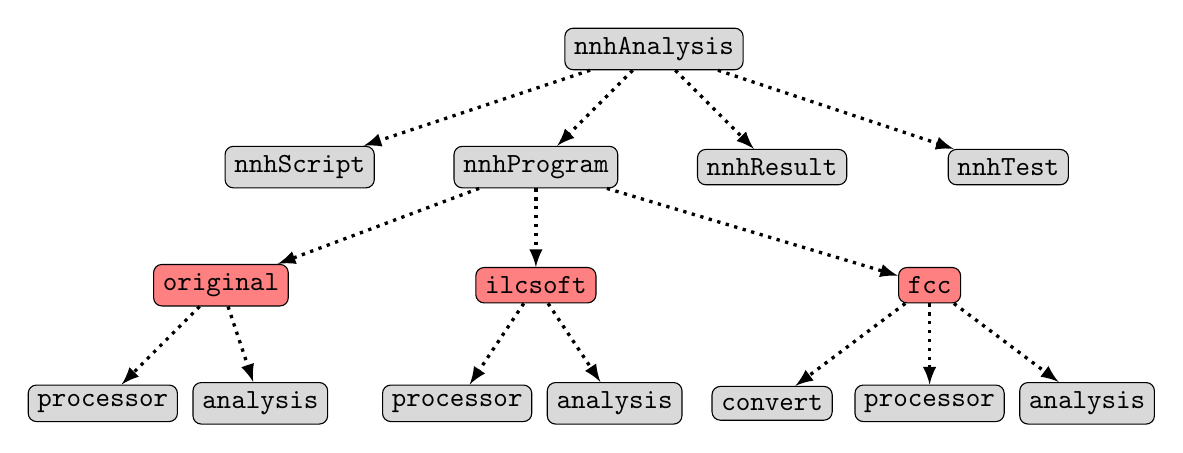
\begin{tikzpicture}
	
		\tikzstyle{home}=[draw, rectangle, fill=red!50, text=black, rounded corners=3pt]		
	
		\tikzstyle{directory}=[draw, rectangle, fill=gray!30, text=black, rounded corners=3pt]

		\node[directory] (A) at (0,0) {\texttt{nnhAnalysis}};
		
		\node[directory] (S) at (-4.5,-1.5) {\texttt{nnhScript}};
		\node[directory] (P) at (-1.5,-1.5) {\texttt{nnhProgram}};
		\node[directory] (R) at ( 1.5,-1.5) {\texttt{nnhResult}};
		\node[directory] (T) at ( 4.5,-1.5) {\texttt{nnhTest}};
		
		\node[home] (O) at (-5.5,-3) {\texttt{original}};
		\node[home] (I) at (-1.5,-3) {\texttt{ilcsoft}};
		\node[home] (F) at ( 3.5,-3) {\texttt{fcc}};
		
		\node[directory] (OP) at (-7,-4.5) {\texttt{processor}};
		\node[directory] (OA) at (-5,-4.5) {\texttt{analysis}};
		
		\node[directory] (IP) at (-2.5,-4.5) {\texttt{processor}};
		\node[directory] (IA) at (-0.5,-4.5) {\texttt{analysis}};
		
		\node[directory] (FC) at (1.5,-4.5) {\texttt{convert}};
		\node[directory] (FP) at (3.5,-4.5) {\texttt{processor}};
		\node[directory] (FA) at (5.5,-4.5) {\texttt{analysis}};
		
		
%		\tikzstyle{files}=[rectangle, draw, fill=red!40, text=black, below right]		
%		
%		\node[files] (r) at (-2.2,-2) {
%				\texttt{...}
%		};
%		\node[files, text width=3cm] (s) at (0.7,-2) {
%				\texttt{nnh.sh}
%				\texttt{nnhProcessor.sh}
%				\texttt{nnhAnalysis.sh}
%				\texttt{prepaeBDT.sh}
%				\texttt{launchBDT.sh}
%				\texttt{nnhExport.sh}
%		};
%		\node[files, text width=5cm] (t) at (4.3,-2) {
%				\texttt{testProcessorCompleted.py}
%				\texttt{testProcessorSame.py}
%				\texttt{testAnalysisCompleted.py}
%				\texttt{testAnalysisSame.py}
%		};
		
		
		\tikzstyle{linkDir}=[->,dotted,very thick,>=latex]
		
		\draw[linkDir] (A)--(P);
		\draw[linkDir] (A)--(R); 
		\draw[linkDir] (A)--(S);
		\draw[linkDir] (A)--(T); 
		
		\draw[linkDir] (P)--(O);
		\draw[linkDir] (P)--(I); 
		\draw[linkDir] (P)--(F);
		
		\draw[linkDir] (O)--(OP);
		\draw[linkDir] (O)--(OA); 
		\draw[linkDir] (I)--(IP);
		\draw[linkDir] (I)--(IA); 
		\draw[linkDir] (F)--(FP);
		\draw[linkDir] (F)--(FA); 
		\draw[linkDir] (F)--(FC);
		
	\end{tikzpicture}
	\caption{
		Organisation des dossiers de mon Projet - \url{https://github.com/alexhxia/nnhAnalysis}
	}
	\label{orga:end}
\end{figure}